% This LaTeX was auto-generated from MATLAB code.
% To make changes, update the MATLAB code and export to LaTeX again.

\documentclass{article}

\usepackage[utf8]{inputenc}
\usepackage[T1]{fontenc}
\usepackage{lmodern}
\usepackage{graphicx}
\usepackage{color}
\usepackage{hyperref}
\usepackage{amsmath}
\usepackage{amsfonts}
\usepackage{epstopdf}
\usepackage[table]{xcolor}
\usepackage{matlab}

\sloppy
\epstopdfsetup{outdir=./}

\begin{document}

\matlabtitle{Simulation analysis $-$ Step response}


\matlabheading{Read the data file and load its data}

\begin{matlaboutput}
TSTOP = 10
\end{matlaboutput}
\begin{matlaboutput}
Tstep = 0
\end{matlaboutput}
\begin{matlaboutput}
stepFinal = 1
\end{matlaboutput}
\begin{matlaboutput}
data = 
    ans: [1x1 timeseries]

\end{matlaboutput}

\matlabheading{Part 01-03 perform step analysis}

\begin{par}
\begin{flushleft}
We calculate the analysis using these intermediate values.
\end{flushleft}
\end{par}

\begin{matlaboutput}
pc10Idx = 8
\end{matlaboutput}
\begin{matlaboutput}
pc90Idx = 12
\end{matlaboutput}
\begin{matlaboutput}
TsIdx = 12
\end{matlaboutput}

\begin{par}
\begin{flushleft}
The results are
\end{flushleft}
\end{par}

\begin{matlaboutput}
stepCharacteristics = 
    peak: 0.2242
    pcOS: 0.8771
      Tr: 0.7997
      Tp: 1.8865
      Ts: 1.0865
     Ess: 0.7778

\end{matlaboutput}

\begin{par}
\begin{flushleft}
Plot the steady state error, followed by the plot with characteristics traced.
\end{flushleft}
\end{par}

\begin{center}
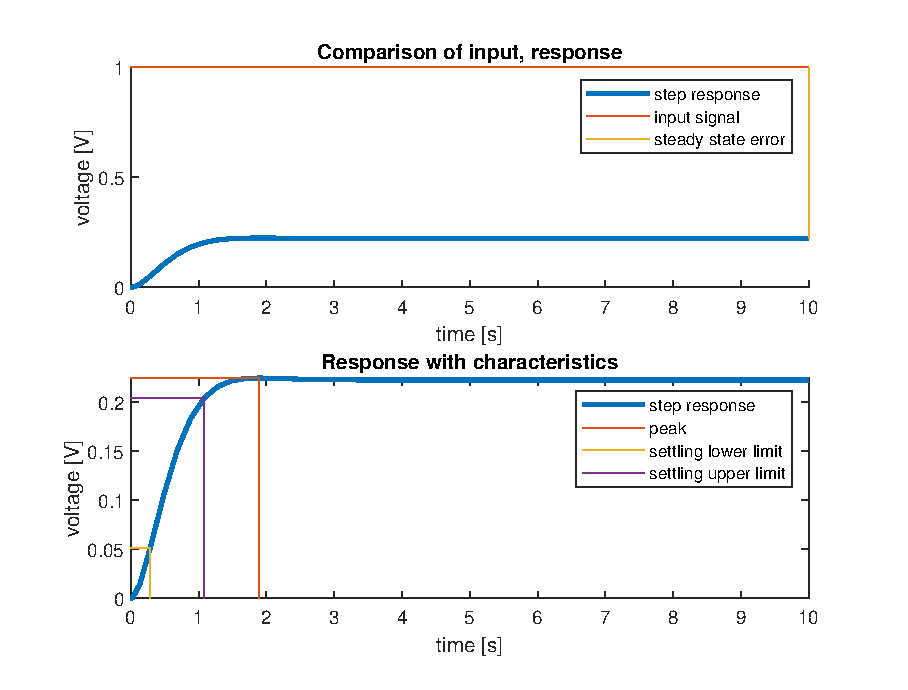
\includegraphics[width=\maxwidth{56.196688409433015em}]{./part01a_step03_simulation_analysis_mlx_images/figure_0.eps}
\end{center}
\end{document}
